\documentclass[10pt, journal]{IEEEtran}
\usepackage{amsmath}
\usepackage{amsfonts}
\usepackage{amssymb}
\usepackage{hyperref}
\usepackage{graphicx}
\graphicspath{ {images/} }
\usepackage[caption=false,font=footnotesize]{subfig}
\usepackage{siunitx}

\makeatletter
\def\endthebibliography{%
  \def\@noitemerr{\@latex@warning{Empty `thebibliography' environment}}%
  \endlist
}
\makeatother

\DeclareMathOperator{\vol}{Vol}
\DeclareMathOperator{\argmax}{argmax}

\title{Boundary-aware Augmentation for Object Detection in Scientific Images
  (DRAFT)}

\author{Benjamin Killeen and Gordon Kindlmann %
  \thanks{Benjamin Killeen is an undergraduate with the Department of Computer
    Science, University of Chicago, Chicago, IL 60637, USA (email:
    \href{mailto:killeen@uchicago.edu}{killeen@uchicago.edu})} %
  \thanks{Gordon Kindlmann is with the Department of Computer Science, 
    University of Chicago, Chicago, IL 60637, USA (email:
    \href{mailto:glk@uchicago.edu}{glk@uchicago.edu})} %
}

\begin{document}
\maketitle

\begin{abstract}
  Recently, deep convolutional neural networks (DCNNs) have enabled remarkable
  progress in computer vision tasks. Given this success, we consider the
  application of DCNNs to image analysis in scientific experiments, which
  traditionally employ time-consuming, \emph{ad hoc} solutions. DCNNs have the
  potential to accelerate this analysis through object detection, but the
  training process for DCNNs requires many labeled images. Crucially, the
  experiment must produce its own training set, and this circularity results in
  over-fitting which violates the scientific method. Unlike object detection for
  real-world tasks, scientific image analysis must be agnostic to
  non-uniformities in the natural world, such as natural laws or governing
  principles. In this report, we introduce boundary-aware augmentation (BAA) as
  an essential component of training DCNNs which agnostic to governing
  principles yet perform reliably on scarce data.\footnote{Code available at
    \href{https://github.com/bendkill/artifice} {github.com/bendkill/artifice}.}
\end{abstract}

\section{Introduction}
\label{sec:introduction}

% TODO: Labeling is perhaps a bad word, limiting to classification. Analysis is
% the word that we might be looking for. Real-valued multivariate descriptions
% of the values captured by those images.

Image analysis is a vital component of many scientific experiments, used to
measure properties like object location or orientation. In cases where no
alternative measuring technique exists, accurate analysis is of the utmost
importance, but this accuracy often proves labor-intensive. Experimenters
utilize \emph{ad hoc} solutions suited for one experimental setup, even though
recent advances in Computer Vision have yielded solutions for seemingly more
general problems.

% TODO: How are we saving the day?
Many factors have contributed to the recent success of DCNNs. In 2012,
Krizhevsky et al. trained a DCNN on the ImageNet dataset, achieving previously
unseen classification accuracy, and showed that state-of-the-art GPUs could
accelerate computation for these kinds of models \cite{krizhevsky_imagenet_2012,
  deng_imagenet:_nodate}. Further advances in computer power continue to
motivate refinements to DCNN design, yielding even higher classification
accuracies \cite{simonyan_very_2014, szegedy_going_2014,
  he_deep_2015}. Meanwhile, datasets with more detailed labels, such as
Microsoft COCO, facilitate supervised training for tasks like bounding-box
detection and instance segmentation \cite{lin_microsoft_2014}. If sufficient
training data exists, DCNNs seem ripe to dramatically accelerate scientific
image analysis.

In general, however, each experiment must produce its own training
data. Ronneberger et al. confront this scarcity for biomedical image analysis
through data augmentation, previously introduced for vision tasks in general,
and network design, introducing a novel DCNN architecture for semantic
segmentation \cite{krizhevsky_imagenet_2012, ronneberger_u-net:_2015}. Another
approach to high-cost labeling is active learning, where a query strategy
selects unlabeled examples which will most benefit training
\cite{settles_active_2012}. Active learning reduces the number of examples---and
thus the man-hours---required for training, making it a vital part of any
workflow with DCNNs for scientific image analysis. For data scarcity in general,
these two approaches, active learning and simple data augmentation, are
sufficient, but data from scientific experiments exhibits not just scarcity but
also undesirable non-uniformity, resulting from general principles.

\begin{figure}
  \centering
  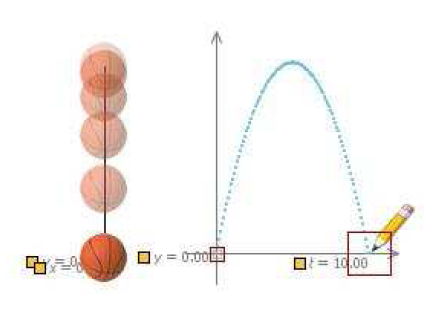
\includegraphics[width=\linewidth]{free_fall}
  \caption{An object in free fall \cite{duquevieira_simple_2012}. (PLACEHOLDER
    IMAGE)}
  \label{fig:free-fall}
\end{figure}

In order to illustrate non-uniformity from general principles, we consider the
concrete example shown in Figure \ref{fig:free-fall}. Here, the experimenter
wishes to study how objects fall, and to do this, he or she has captured images
at regular intervals of a basketball in free-fall. Because objects accelerate
downward at a constant rate of approximately 9.8 \si{\meter\per\second^2}
\cite{munroe_wikipedian_nodate}, her data will consist of many more examples
with the basketball in the top half of the image than the bottom. This uneven
distribution comprises a ``non-uniformity,'' and the natural law it results from
is a \emph{governing principle}. As a matter of course, the experimenter may
have hypothesized that this principle exists, but according to the scientific
method, should not incorporate her hypothesis into her measurement. This
complication presents a challenge for training a DCNN---or any predictive model,
for that matter---with data from the experiment itself. The distribution of $y$,
shown in Figure \ref{fig:free-fall}, should not influence future measurements of
$y$.

% TODO: think about splitting up these figures? The reader will want to know
% what you're doing differently. Without a figure and with words alone, describe
% broadly what you're doing in the intro. Also: export to PDF and not PNG.

\begin{figure*}
  \centering
  \subfloat[]{
    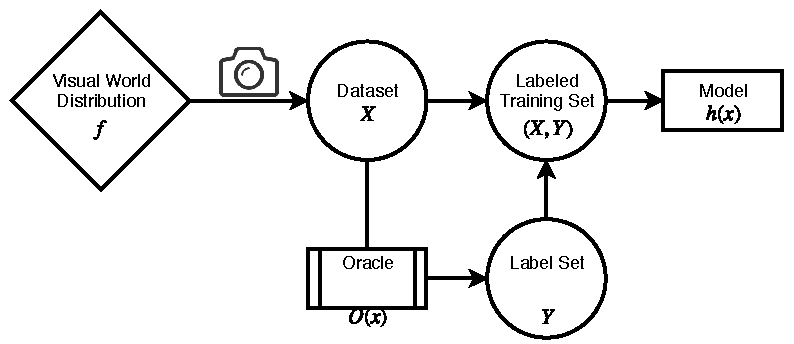
\includegraphics[width=0.46\linewidth]{traditional_graph}
    \label{fig:traditional-graph}
  }
  \hfill
  \subfloat[]{
    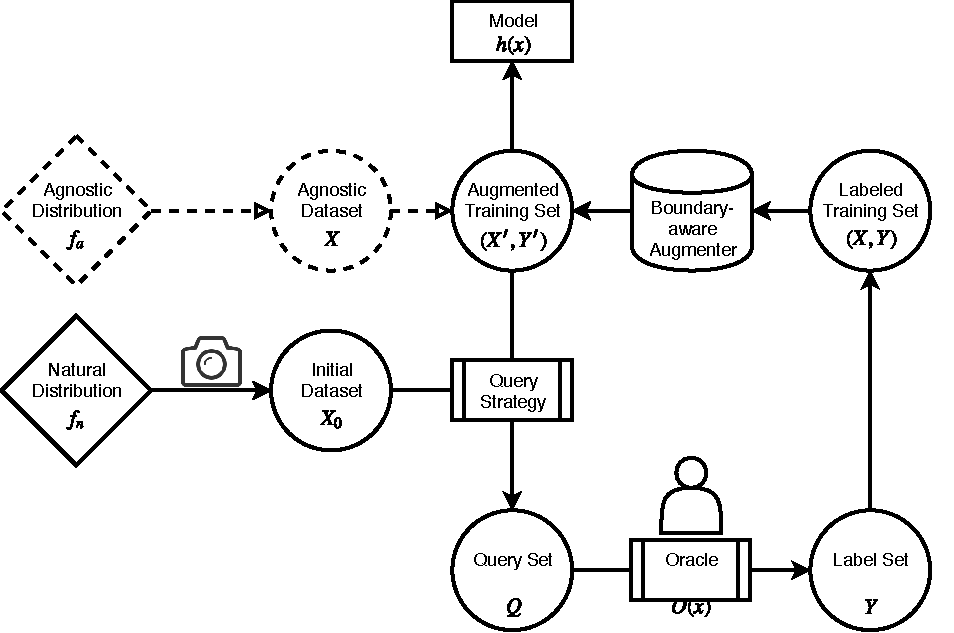
\includegraphics[width=0.50\linewidth]{artifice_graph}
    \label{fig:artifice-graph}
  }
  \caption{During supervised learning for real-world vision tasks \textbf{(a)},
    a camera samples a large dataset $X$ from the ``visual world'' distribution
    $f$. For scientific tasks \textbf{(b)}, an experiment samples a small
    initial dataset $X_0$ from the natural distribution $f_n$, which includes
    the effects of any governing principles. Our proposed training method
    incorporates a boundary-aware augmenter $A$, which uses the training set
    $(X,Y)$ to simulate drawing examples from the agnostic distribution
    $f_a$. Dashed lines indicate theoretical or simulated objects.}
  \label{fig:dependency-graphs}
\end{figure*}

Unfortunately, a DCNN can incorporate that distribution into its parameters
during learning. This makes it more likely to predict images with the basketball
in the top half of the image than the bottom. It could also fail to capture any
anomalies in the basketball's trajectory, if gravity didn't behave the way we
expect. Ideally, therefore, we would sample the training set from a
universe---so to speak---where gravity doesn't affect the basketball's
position. The question immediately arises: how does the ball behave in this
universe? Or rather, how \emph{should} the ball behave? Because we wish to
create a DCNN for object detection, we should sample position as uniformly as
possible.

To formalize these ideas, we contrast between traditional and scientific vision
tasks. Figure \ref{fig:traditional-graph} outlines the training process for
supervised learning. It begins with a large, ordered dataset
$X \subseteq mathbb{R}^{M \times N}$ of $M \times N$ images, sampled from the
``visual world.'' Next, an oracle
$O : X \subseteq mathbb{R}^{M \times N} \rightarrow \mathbb{R}^n$ (usually a
human) provides the label set $Y = \{O(x) : x \in X\}$, where $n$ is the
dimensionality of the labels, \emph{e.g.} number of classes in a one-hot
encoding. In any task, this label is a lower-dimensional representation of
the data space, encoding valuable information from each example. Together, the
data and label sets $(X,Y)$ comprise the training set. Supervised learning
aims to train a model (such as a DCNN)
$h : \mathbb{R}^{M\times N} \rightarrow \mathbb{R}^n$ that can interpret the
visual world. Crucial, the visual world is not a uniformly distributed set of
images; we denote its probability distribution as
$f : \mathbb{R}^{M\times N} \rightarrow \mathbb{R}$, from which every dataset
draws examples as independently and identically distributed as possible (or
attempts to).

For real-world tasks, sampling $f$ in this manner is desirable, but in
scientific tasks, $f$ contains the effects of governing principles. Instead, we
wish to sample a dataset $X$ that correspond to labels $Y$ as uniform as
possible---within reasonable boundaries---in the label space
$\mathbb{R}^n$. Incidentally, most scientific experiments have well-known
\emph{label-space boundaries} incorporated into their design. A ball on a
ramp, for instance, is bound to one dimension, even though its image-space
position is described by two coordinates. Figure \ref{fig:gyros} shows an
experiment where dot markers are confined to a small circular region. The region
$\psi \subseteq \mathbb{R}^n$ that these boundaries define corresponds to a
higher-dimensional data-space region $\chi \subseteq \mathbb{R}^{M\times N}$
such that the real distribution $f$ obeys
\[ (\forall x \not\in \chi)(f_n(x) = 0). \] Note that $\chi$ is not necessarily
the smallest such space; the experimenter simply determines reasonable
boundaries for $\psi$ such that the above condition is satisfied. Even with
perfect knowledge of $\psi$, it would be impossible to recover
$\chi$. Nevertheless, we will attempt to do just that.

Although $\chi$ is largely a theoretical construct, it serves as a useful
concept for training models which are agnostic to governing principles. Consider
the uniform distribution across it, which we will refer to as the \emph{agnostic
  distribution}:
\[ f_a(x) =
  \begin{cases}
    \frac{1}{\vol(\chi)} & x \in \chi \\
    0 & x \not\in \chi
  \end{cases}
\] From the initial dataset $X_0$, then, we wish to generate and label an
augmented dataset $X$ that approximates an agnostic dataset $X_a \sim f_a$. For
this purpose, we introduce \emph{boundary-aware augmentation} (BAA), which
utilizes the label-space region $\psi$ and instance segmentations to approach
$X_a$. We further denote the label-space uniform distribution
\[ g_a(y) =
  \begin{cases}
    \frac{1}{\vol(\psi)} & y \in \psi \\
    0 & y \not\in \psi,
  \end{cases}
\] the lower-dimensional representation of $f_a$.

% TODO: just put citations at the end of the sentence, sentence should stand
% alone.

\section{Method}
\label{sec:method}

With practical application in mind, we outline our method as it relates to an
active learning strategy with an on-line oracle, \emph{i.e.} a human. The query
strategy is a vital part of any system utilizing our method, but its final form
will depend on the exact details of our implementation. We rely on existing
literature for inspiration, but for the time being, we may consider a query
strategy which selects unlabeled images either at random or according to
uncertainty \cite{settles_active_2012, vezhnevets_active_2012}.

The function of our augmentation scheme, BAA, is more fundamental. Like any data
augmentation scheme, it aims to mitigate the effects of data scarcity, which
\cite{krizhevsky_imagenet_2012} achieves through image-global transformations
such as flipping and brightness shifts. In order to address governing
principles, however, our augmentation scheme must be able to generate examples
$x$ from arbitrary points $y$ in label space $\mathbb{R}^n$. In principle, the
label space can include a large number of object properties which the
experimenter wishes to measure, including position in the image, apparent
orientation, size, and any number of one-hot classifications. These apply to
every object in the image, resulting in a label space that can grow relatively
large, with independent boundaries on $\psi$ for every coordinate. For the
following explanation, we consider a label space of object positions, but
maintain that the same principles apply for higher-dimensional label spaces.

% TODO: figure illustrating segmentation augmentation?
In order to freely manipulate examples in label-space, we introduce an
intermediate \emph{annotation space} $\mathbb{R}^{M\times N \times k}$ between
the data and the labels, where $k$ is the dimensionality of the
annotation. Although the specific details of the annotation space are still
under consideration, it includes an instance segmentation of the image $x$. With
this information, BAA can extract the pixels belonging to every object in the
image and translate them freely. Unlike image-global strategies, this method
directly addresses the label-space representation of an example. It also raises
two questions: what pixels should the augmenter use to replace the extracted
object, and what new points in label-space should the augmenter introduce? The
first question is a matter of practical importance, but the second directly
relates to our primary goal.

% TODO: figure illustrating inpainting?
There are many possible solutions to the problem of pixel-replacement. Most
simply, one could use the mean value of the surrounding region, or else gaussian
noise with the same mean and standard deviation. \cite{bertalmio_image_2000}
describes a more nuanced approach that attempts to complete isophote lines
arriving at the region's edge. \cite{pathak_context_2016} introduces Context
Encoders: DCNNs that incorporate the entire image to inpaint a desired
region. Any of these methods should prove effective for our purposes, although
in many cases they may prove unnecessary. Many scientific tasks are the result
of fixed-camera video data. If another example in the labeled dataset includes
background pixels from the desired region, then the most effective approach
would simply ``transplant'' these pixels, so to speak, from that example.

Once an object-region has been extracted, the question of placement depends on
how uniformly $Y$ covers $\psi$. By placing new examples properly (and
potentially removing old ones) BAA should generate $X'$ that more uniformly
covers $\chi$. This requires a comparison of the multivariate sampling $Y$ with
the multivariate distribution $g_a$, so we denote similarity function $S$ to
perform this comparison. For the time being, the choice of $S$ is unclear, but
possible choices include a coordinate-wise Kolmogorov-Smirnov test. Although
this is not a general solution in the multivariate case, it is perfectly
acceptable when $\psi$ is bounded by affine subspaces. Additionally, Justel et
al. describe a variation of the K-S test which can be efficiently approximated
in high dimensions \cite{justel_multivariate_1997}. In any case, we wish to
generate labels $Y'$ such that
\[ Y' = \underset{Y' | Y \subseteq Y'}{\argmax} S(Y', g_a). \] After placing
extracted objects, this yields an augmented dataset approximating
$X_a \sim f_a$.

\section{Evaluation}
\label{sec:evaluation}

\begin{figure}
  \centering
  \subfloat[Gyroscopic Model]{
    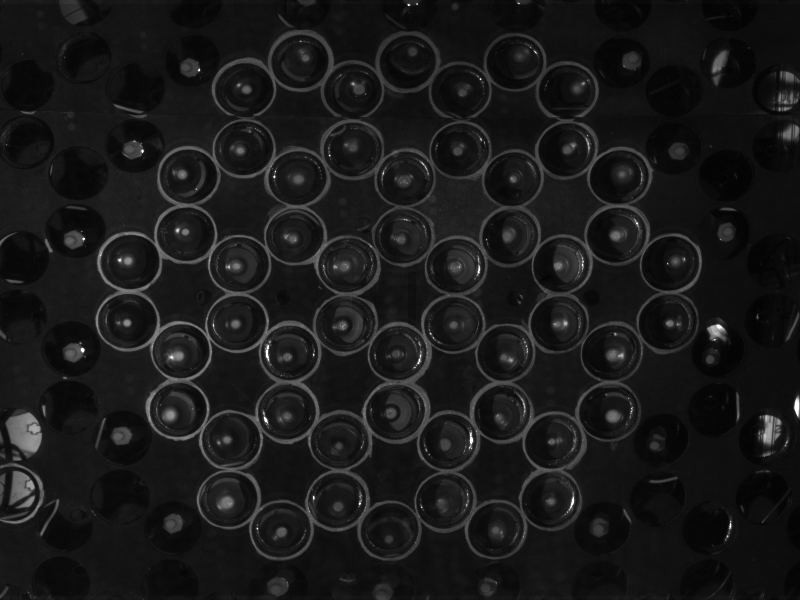
\includegraphics[height=0.37\linewidth]{gyros}
    \label{fig:gyros}
  }
  \hfill
  \subfloat[Coupled Spheres]{
    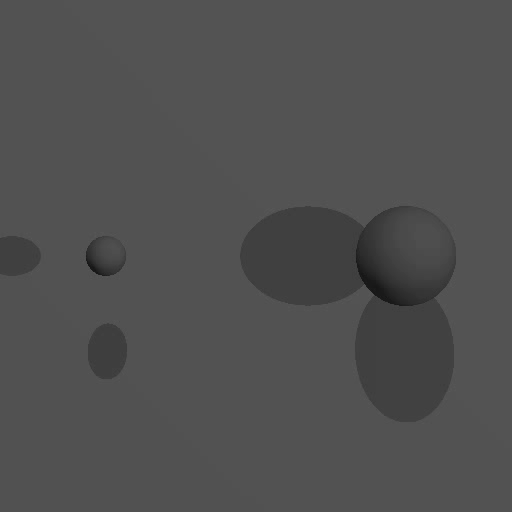
\includegraphics[height=0.37\linewidth]{coupled_spheres}
    \label{fig:coupled-spheres}
  }
  \caption[example experiments]{Example images from scientific experiments:
    \textbf{(a)} gyroscopic model for topological metamaterials
    \cite{nash_topological_2015}. Each dot is bound inside the circle
    surrounding it. \textbf{(b)} still frame from a simulated experiment of two
    spheres coupled by an invisible spring. Full video \href
    {https://github.com/bendkill/artifice/blob/master/docs/coupled_spheres.gif}
    {here}.}
  \label{fig:example-experiments}
\end{figure}

In order to show our method's effectiveness, we develop several virtual
experiments. These simulations offer several advantages over images from real
experiments, such as in Figure \ref{fig:gyros}. First, we have perfect knowledge
of the experiment's ``Truth'' $\tilde{Y}$, as opposed to imperfect measurements,
or ``ground truth,'' $Y$. In well established datasets, $\tilde{Y}$ and $Y$ are
nearly identical, but we must rely on one or a few human labelers for what
should be unambiguous quantities. For testing, we calculate $\tilde{Y}$ from the
known parameters of the simulation, and we emulate a human labeler by
introducing small perturbations to $\tilde{Y}$, producing $Y$. Part of our goal
is to train a DCNN that more closely predicts $\tilde{Y}$ than the labels
$Y$. Simulated experiments allow us to test this performance.

Figure \ref{fig:coupled-spheres} shows one such experiment. In this case, two
spheres with different masses rotate in free space, coupled by an invisible
spring. The goal of the Coupled Spheres experiment is to recover physical
properties of the spring using $(x,y)$ positions of the two spheres. These
physical properties comprise the general principles underlying the dataset. To
evaluate our method's agnosticism toward general principles, we intend to train
a DCNN on one experiment and evaluate its performance on experiments with
different simulated springs. This simple example illustrates the general
resilience that we wish to develop.

\section{Discussion}
\label{sec:discussion}

We have illustrated the problem of applying predictive models like DCNNs to
scientific images without proper care. We have proposed a method, boundary-aware
augmentation, that addresses this issue by considering a uniform distribution
over the data region $\chi$. Although this method is (in theory) successful in
created an augmented dataset which is agnostic to general principles, the
resulting dataset $X$ is also agnostic to any other non-uniformities in
$X_0$. We have also not addressed the reasonable constraint of temporal
continuity. Instead, we chose to consider isolated frames with an
\emph{arbitrary} rather than \emph{temporal} ordering, but we could consider
instead the uniform distribution of paths that an object could take from one
frame to the next, within some reasonable maximum.

% TODO: not in the paper, ignoring everything, all of law's natures, in addition
% to GPs

% TODO: think about time, how are we treating the chronological ordering of the
% data?

% TODO: it's okay for the object to have some notion of continuity. The
% experimenter knows the max velocity that these things could have, puts a cap
% on the maximum distance between examples.

\section*{Acknowledgment}
\label{sec:acknowledgment}

Thanks to Michael Maire for input and guidance, as well as William Irvine for
access to image data from his laboratory.

\bibliographystyle{IEEEtran}
\bibliography{report}

\end{document}
%%% Local Variables:
%%% mode: latex
%%% TeX-master: t
%%% End:
